\documentclass{report}

\setlength{\textwidth}{150mm}
%\setlength{\textheight}{195mm}
\setlength{\oddsidemargin}{9mm}
%\setlength{\evensidemargin}{28mm}
%\setlength{\topmargin}{-10mm}


\usepackage[utf8]{inputenc}
\usepackage{graphicx}
\graphicspath{ {images/} }
\usepackage{caption}
\usepackage{subcaption}
\usepackage{wrapfig}

\begin{document}
\begin{titlepage}
\centering

\begin{figure}[t]
\includegraphics[scale=0.5]{images/urjc_logo.png}
\centering
\vspace{0.5cm} %Espacios despúes de la imagen
\end{figure}

{\scshape\Large Escuela Técnica Superior de Ingeniería de Telecomunicación \par}
\vspace{1cm}
{\scshape\Large Grado en Ingeniería en Sistemas de Telecomunicación \par}
\vspace{3cm}
{\bfseries\LARGE DeepLearning y procesamiento de imagen en un robot educativo simulado
en navegador web\par}
\vspace{3cm}
{\itshape\Large Trabajo fin de grado \par}
\vfill
{\Large Autor: }
{\Large Jorge Cruz de la Haza \par}
{\Large Tutor: }
{\Large Dr. Jose María Cañas Plaza \par}
{\Large Co-Tutor: }
{\Large Prf. Julio Manuel Vega Pérez \par}
\vfill
{\Large Curso Académico 2019/2020 \par}
\end{titlepage} 

\renewcommand{\abstractname}{\Large Resumen}
\begin{abstract}
Hablar de Robótica, Kibotics y la ciudad simulada.


\end{abstract}

\setcounter{tocdepth}{3} %Para que aparezcan las subsubsection{}
\renewcommand{\contentsname}{Índice general}
\tableofcontents
\clearpage

\renewcommand{\listfigurename}{Índice de figuras}
\listoffigures

\renewcommand{\listtablename}{Índice de tablas}
\listoftables

\renewcommand{\chaptername}{Capítulo}
\chapter{Introducción}

En este capítulo se expone el contexto general que envuelve este proyecto, así como situarlo dentro del mismo. Se explica qué es la robótica, el Deep Learning (o aprendizaje profundo) en visión artificial y, al mismo tiempo, la importancia que va cobrando cada vez más la robótica en la educación. Finalmente se presentarán algunas plataformas robóticas educativas interesantes, así como la plataforma utilizada para este proyecto. En concreto esta plataforme se 

\section{Robótica}

Isaac Asimov fue un escritor ruso, cuya obra principal se basó en la ciencia ficción, la historia y la divulgación científica. Debido a la gran cantidad de publicaciones relacionadas con los robots (de ficción y no ficción) es considerado como \textit{El Padre de la robótica}. En 1950 publicó \textit{''Yo, Robot''}, una colección de relatos que tratan sobre robots inteligentes, y en los que Isaac predijo el aumento de la industria de la robótica. El origen de la palabra robot proviene de la palabra eslava \textit{robota}, que hace referencia al trabajo que se realiza de manera forzada. 
\\

Hoy en día la robótica hace referencia a la disciplina cietífica que aglutina distintas ramas tecnológicas (como la mecánica, la física, las matemáticas, o la inteligencia artificial), con el propósito de diseñar máquinas robotizadas (robots) que sean capaces de realizar tareas de manera autónoma. El objetivo del diseño de estas máquinas es poder facilitar la vida de las personas y, en algunos casos, llegar a sustiturlas en algunos trabajos. Las aplicaciones de la robótica pueden llegar a ser realmente útiles en las tareas cotidianas y son de especial interés  cuando los robots pueden simular el comportamiento humano en tareas que puedan suponer un riesgo para las personas, evitando así que estas corran ese riesgo.
\\

Existen diferentes tipos de clasificaciones de robots entre las que podemos encontrar:

\begin{enumerate}
	\item En función de su utilidad:
	\begin{itemize}
		\item Industriales. Son aquellos que están destinados a realizar determinados procesos o tareas de una forma automática, principalmente orientados a procesos de fabriación o manufacturación. Se caracterizan por tener brazos mecánicos o poliarticulados con distintos ejes, que pueden ser móviles o fijos. Estos tipos de robots no necesitan la manipulación de una persona para realizar su tarea.
		
		\item Móviles. Disponen de mecanismos que les permiten desplazarse, siguiendo un camino teleoperado o identificando los elementos de su entorno y desplazándose de manera autónoma. Son útiles para el transporte, cadenas de fabricación, envíos, etc. Se caracterizan por tener un relativo elevado nivel de inteligencia.
		
		\item Médicos. Destinados a realizar distintas funciones aplicadas al ámbito de la medicina, tales como robots que permitan escanear información del cerebro, robots con medidas de precisión que indiquen el punto exacto donde hay que realizar una incisión para una operación, telediagnóstico o telecirugía. Recientemente está en auge la industria robótica dedicada a fabricar prótesis dotadas de sistemas de mando que permiten simular los movimientos y funciones de los órganos.
		
		\item Androides. Son quellos fabricados con apariencia y características similares a los humanos. Imitan acciones o conductas de las personas de manera autónoma. A día de hoy este tipo de robots no está muy evolucionado debido a que resulta complicado emular y coordinar los movimientos y comportamientos humanos. Dentro de este grupo se incluyen los robots zoomórficos, que se caracterizan por imitar los movimientos y características de distintos seres vivos.
		 
		\item Híbridos. El resto de robots que no pueden clasificarse en ninguna de las categorías anteriores o que presentan características de dos o más categorías al mismo tiempo.

\renewcommand{\figurename}{Figura}		
\begin{figure}[h]
\centering
  \begin{subfigure}[b]{0.25\textwidth}
    \includegraphics[width=\textwidth, height=\textwidth]{images/robot_industrial.png}
    \caption{Robot industrial}
    \label{fig:f1}
  \end{subfigure}
    \begin{subfigure}[b]{0.25\textwidth}
    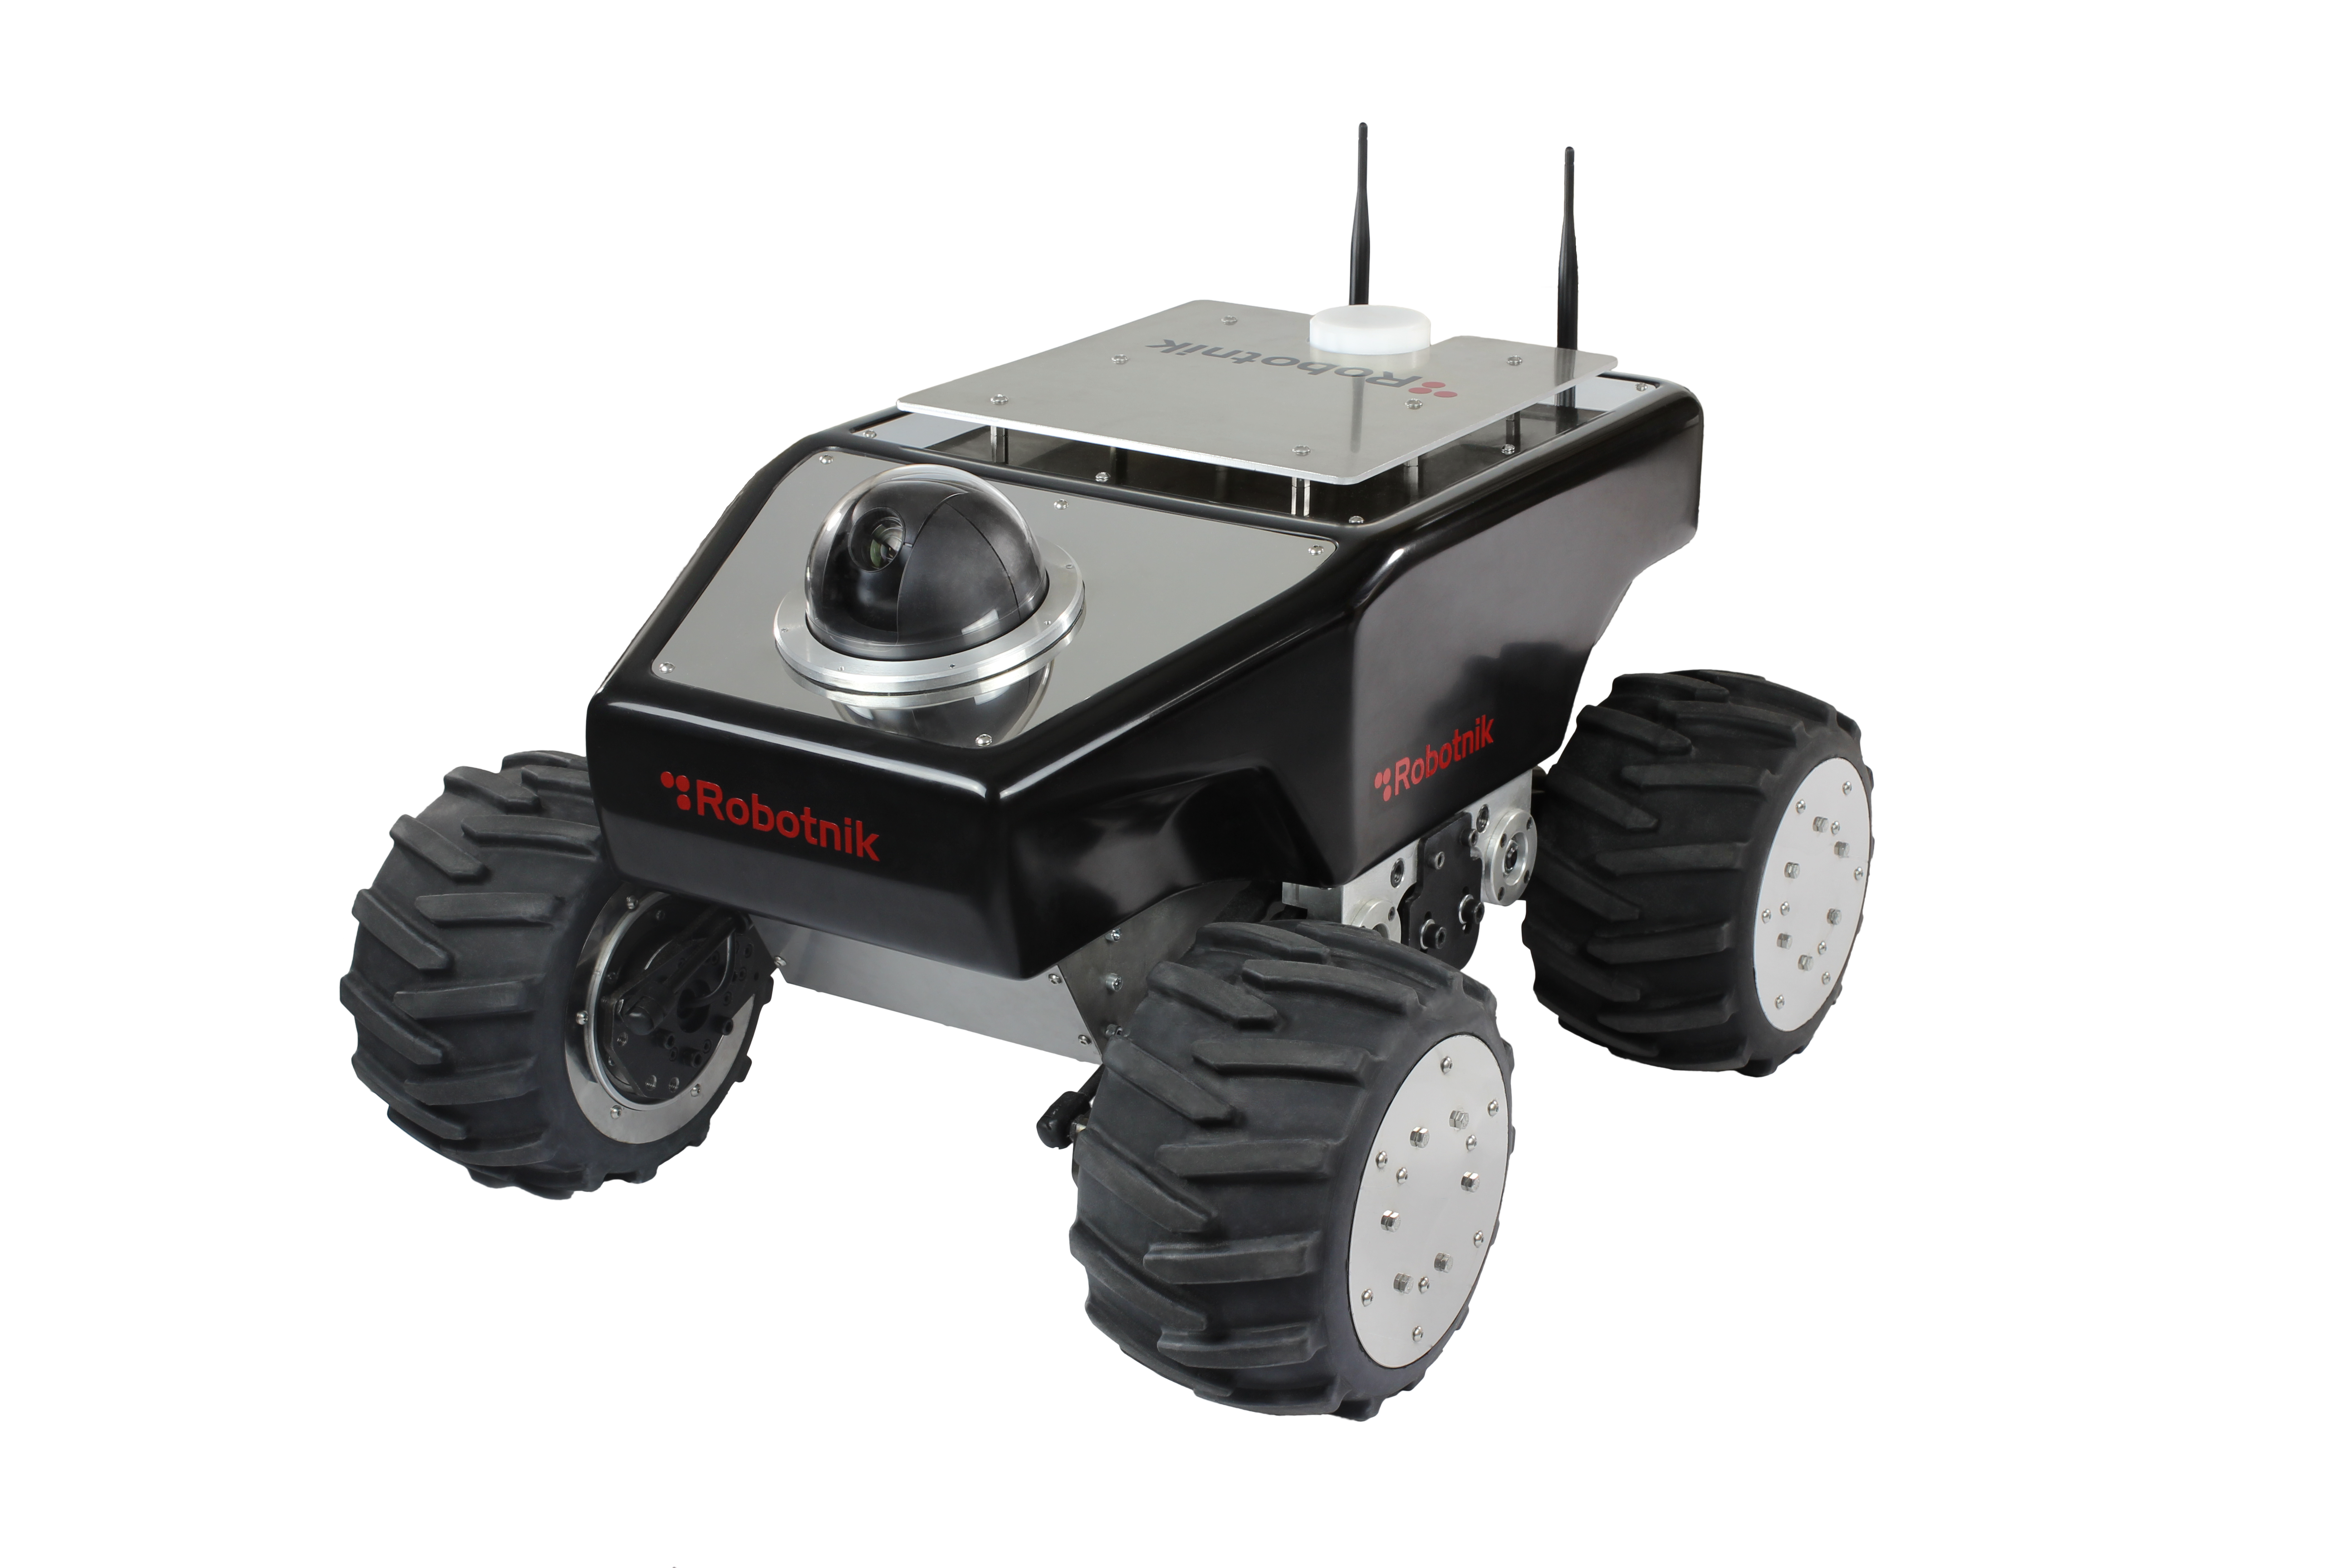
\includegraphics[width=\textwidth, height=\textwidth]{images/robot_movil.png}
    \caption{Robot móvil}
    \label{fig:f2}
  	\end{subfigure}
  	\begin{subfigure}[b]{0.25\textwidth}
    \includegraphics[width=1.3\textwidth, height=\textwidth]{images/robot_medico.png}
    \caption{Robot médico}
    \label{fig:f3}
  	\end{subfigure}
  	\begin{subfigure}[b]{0.25\textwidth}
    \includegraphics[width=0.7\textwidth, height=\textwidth]{images/robot_androide.png}
    \caption{Robot androide}
    \label{fig:f3}
  	\end{subfigure}
  	\caption{Tipos de robots en función de su utilidad.}
\end{figure}
	\end{itemize}


	\item En función de su operación:
	\begin{itemize}
		\item Robots teleoperados. Aquellos robots cuyas acciones que son controladas de manera remota por una persona. Este tipo de robots se utilizan principalmente en tareas que puedan suponer un riesgo de salud para las personas, pero que al mismo tiempo requieran un tratamiento humano para su elaboración (por ejemplo, robots para desactivación de bombas).
		
		\item Robots autónomos. Por el contrario, este tipo de robots son capaces de realizar taeras de manera independiente ya que son máquinas mucho más complejas y son dotadas con cierta inteligencia. Este tipo de robots son utilizados en algunos escenarios en los que el robot es capaz de analizar el entorno que le rodea para generar una respuesta por sí mismo. Este tipo de robots es el que utilizaremos para desarrollar este proyecto.
	\end{itemize}
\end{enumerate}

A día de hoy existen numerosas aplicaciones de la robótica en nuestra vida cotidiana, y cada vez son más los casos de uso debido a su gran utilidad y a la mejora que producen en la vida de las personas. El campo de la robótica está en continuo investigación y desarrollo, debido en gran parte a la gran velocidad con la que ha avanzado la tecnología en los últimos años. Algunos de los ejemplos más relevantes del uso de la robótica en nuestra vida cotidiana son; el coche autónomo de Tesla, dotado de cámaras y sensores que permiten que el coche sea capaz de circular de manera autónoma e identificar su entorno para actuar en consecuencia (detenerse en caso de que haya un peatón justo en frente, corregir la trayectoria en caso de pisar una línea continua…);  aspiradoras Roomba, capaces de identificar y memorizar la superficie aspirada para recorrer  y limpiar toda la vivienda de manera autónoma;  el robot DaVinci, un instrumento quirúrgico capaz de reproducir los movimientos de un cirujano sin latencia y con precisión, que permite reducir los temblores del cirujano y hace que pueda operar sentado de una manera más cómoda; centros logísticos de Amazon equipados con robots que ayudan a los humanos a seleccionar, clasificar, transportar y almacenar paquetes.
\\

Sin duda la robótica es un campo muy útil, en continuo desarrollo y de gran interés común, por lo que realizar un trabajo de fin de grado en este ámbito resulta interesante ya que es un tema que está a la orden del día y son muchos los casos de uso realizables en la vida real.


\section{Deep Learning en Visión Artifical}
Muchos de los robots actuales tienen una cámara como sensor principal que les permite tener cierto conocimiento del entorno en el que se encuentran, por lo que pueden actuar e interaccionar con los elementos que les rodean en consecuencia. Por tanto, estos robots se convierten en sistemas inteligentes cuya inteligencia está dotada principalmente por dos elementos: la cámara (visión artificial) y los algoritmos que procesan esas imágenes (Deep Learning).
\\

El \textit{Deep Learning} (aprendizaje profundo) es una rama de la ingeniería que permite a un ordenador crear conceptos y lógicas complejas a partir de otras más simples, todo ello mediante un aprendizaje automático. Los algoritmos de DeepLearning permiten crear un conocimiento en una máquina mediante un entrenamiento e intentan modelar abstraciones de alto nivel (por ejemplo, percepciones humanas tales como identificar distintos objetos en una imagen) utilizando arquitecturas compuestas de transformaciones no lineales múltiples. Una de las grandes ventajas del Deep Learning es que, a medida que aumenta la cantidad de datos y de ejemplos utilizados, mejora la precisión del algoritmo.
\\

En un contexto más amplio, el \textit{Deep Learning} es una familia de técnicas dentro del Aprendizaje Automático, que es parte de la Inteligencia Artificial (IA). La IA que es la ciencia que estudia la inteligencia que es capaz de desarrollar una máquina mediante la programación. Dentro de la Inteligencia Artificial podemos encontrar el Aprendizaje Máquina (\textit{Machine Learning}), definido como la capacidad de las máquinas para aprender, construyendo modelos o patrones a partir de datos no procesados); el Aprendizaje de la Representacion (\textit{Representation Learning}), que emplea el Aprendizaje Máquina para descubrir automáticamente representaciones o clasificaciones de datos sin procesar); y el Aprendizaje Profundo (\textit{Deep Learning}). En partircular, el Deep Learning se caracteriza por ofrecer muy buenos resultados en detección de objetos en imágenes. El diagrama de Venn (Figura 1.2) muestra los subconjuntos de la Inteligencia Artificial.
\\

Por otra parte, la Visión Artificial (\textit{Computer Vision}) es la rama de la ciencia que recopila todos los métodos para adquirir, procesar, analizar y comprender las imágenes del mundo real para que puedan ser procesadas por un ordenador. En concreto, en este proyecto combinaremos la visión artificial para obtener imágenes de un robot en un entorno real simulado y el \textit{Deep Learning}, para el procesamiento e interpretación de esas imágenes y así dotar de cierta inteligencia necesaria al robot para que sea capaz de actuar en función de las condiciones de su entorno. 

\renewcommand{\figurename}{Figura}		
\begin{figure}[h]
	\centering
	 \includegraphics[scale=0.5]{images/diagrama-venn.jpg}
	 \caption{Diagrama de Venn}
\end{figure}

\newpage
\subsection{Redes Neuronales Convolucionales (CNNs)}

Existen distintas técnicas para llevar a la práctica el \textit{Deep Learning}. Una de ellas son las Redes Neuronales Convolucionales (CNN). Las redes neuronales son modelos de aprendizaje automático que intentan emular las neuronas de los sistemas nerviosos biológicos. Al igual que un cerebro humano, las redes neuronales pretenden establecer conclusiones de los datos que obtienen. En concretro, las Redes Neuronales Convolucionales utilizan filtros convolucionales (múltiples filtros o capas por los que va pasando la información) para realizar esta función.
\\

La arquitectura de las Redes Neuronales Convolucionales se basa en utilizar distintos niveles o capas en los que despúes de cada uno de ellos se añade una función para realiar un mapeo causal no-lineal. Es decir, cada capa está formada por dos subcapas: una capa convolucional (que realiza una operación de convolución), y una capa de submuestreo (\textit{pooling}, que genera características a partir de cálculos estadísticos del resultado de la convolución). Todas estas capas están conectadas de  tal forma que a la salida de todas ellas se puedan obtener conclusiones a partir de los resultados obtenidos. Cuantas más capas posea una red neuronal, más probabilidad hay de que los resultados obtenidos sean acertados. En la Figura 1.3 podemos encontrar un ejemplo de una red neuronal convolucional que clasifica un número manuscrito al número digital que corresponde. 

\renewcommand{\figurename}{Figura}		
\begin{figure}[h]
	\centering
	 \includegraphics[scale=0.45]{images/ejemplo_cnn.png}
	 \caption{Ejemplo de la arquitectura de una Red Neuronal Convolucional}
\end{figure}

Este trabajo se centra en la detección de objetos a través de imágenes, por lo que las Redes Neuronales Convolucionales son de gran utilidad ya que con ellas se puede procesar la imagen por secciones e identificar los objetos de manera más eficiente. Aplicando una red neuronal convolucional a nuestras imágenes podremos identificar el tamaño, la posición y el tipo de objeto que aparece en una imagen, siempre y cuando la clasificación del objeto identificado se encuentre dentro de las clases determinadas de la red neuronal. Para dicha implementación existen diversas plataformas tales como \texttt{Keras}, \texttt{TensorFlow}, \texttt{Caffe}, etc. En nuestro caso utilizaremos \texttt{TensorFLow} y, en concreto, TensorFlowjs, que es la librería para desarollarlo en JavaScript. El motivo de esta elección es que utilizaremos nuestra red en un entorno web, por lo que el hecho de que exista dicha librería en lenguaje JavaScript nos facilitará la incorporación de la red a nuestro entorno. Además, TensorFlow dispone de numerosos modelos pre-entrenados que podremos usar sin la necesidad de entrenar previamente un modelo y etiquetar infinidad de imágenes.

Algunos ejemplos en la vida real de la aplicación de Deep Learning y redes neuronales en procesamiento de imágenes son; Google Photos y su algoritmo para reconocer rostros y organizar las imágenes de la galería; reconocimiento inteligente de defectos en las piezas de una fábrica a través de una cámara que va captando las piezas que pasan a través de una cinta; la creación de ImageNet, una base de datos de imágenes clasificadas cuya creación se ayudó de técnicas de DeepLearning para clasificar las imágenes; Autopilot, la función de conducción autónoma de los coches Tesla que utiliza algoritmos de Deep Learning para materializar las abstracciones de su entorno y poder identificar los objetos que rodean al coche en todo momento y lograr así una conducción autónoma. 

\section{Robótica en educación}

En virtud del auge que está sufriendo la robótica en los últimos años, cada vez son más los profesionales demandados en este campo. Debido a esto, en paralelo con el auge de la robótica, también ha aumentado de manera exponencial la enseñanza de la róbotca en edades tempranas ya que apreder robótica puede ofrecernos una formación en diversos campos de forma simultánea: física, electrónica, informática...Además, el uso de aplicaciones de robótica refuerza la creatividad (a través del diseño de ideas y su desarrollo), el pensanmiento crítico (pensamientos lógicos) y prepara a los niños para un futuro en el que la robótica adquirirá un papel fundamental en la sociedad. Poco a poco se han ido introdución materias de robótica en la enseñanza. Por ejemplo, en la Comunidad de Madrid y en muchas otras se ha incluido en los proyectos formativos asignaturas de robótica. En contexto universitario se han creado grados específicos de robótica, como el grado de robótica en la Universidad de Alicante o el Grado en ingeniería robótica en la Universidad  Rey Juan Carlos. Además, en estos últimos años se han desarrollado numerosas plataformas orientadas a este fin. Entre ellas podemos encontrar OpenRoberta, iRobot y Kibotics (que es la que usaremos para este proyecto). A continuación se detallan cada una de ellas.

\subsection{OpenRoberta}

Es una plataforma \footnote{https://lab.open-roberta.org/} orientada a la programación por bloques en la que se pueden programar robots y otros sistemas hardware programabes como \texttt{Arduino}, \texttt{BBC micro} y \texttt{Calliope mini}. El objetivo de OpenRoberta es simplificar los conceptos de programación para poder introducir esta materia en los colegios. Ofrece un entorno de programación basado en la nube y desarrollado en código abierto que permite su uso en cualquier navegador sin necesidad de instalación. Dispone de varios robots y sistemas (mBot, Arduino,etc) con múltiples motores y sensores que pueden ser configurados a través de bloques. Ofrece múltiples idiomas y no es necesario registrarse para utilizarlo.

\renewcommand{\figurename}{Figura}		
\begin{figure}[h]
	\centering
	 \includegraphics[scale=0.34]{images/openRoberta.jpg}
	 \caption{Interfaz de OpenRoberta}
\end{figure}

\newpage
\subsection{iRobot Education}

iRobot es una empresa estadounidense que se dedica al diseño y fabricación de robots, principalmente orientados al uso en empresas, hogares e instituciones. Es conocida por el robot \textit{Roomba}, una aspiradora doméstica inteligente. Esta empresa ha creado iRobot Education \footnote{https://edu.irobot.com/}, una plataforma educativa destinada al aprendizaje de robótica. Esta empresa comercializa distintos robots, como por ejemplo el  robot móvil llamado \texttt{Create2}, muy parecido a su famoso aspirador Roomba, que los estudiantes y desarrolladores pueden programar para controlar los movimientos y el comportamiento del mismo de una manera sencilla a través de su plataforma. Otro robot que comercializan es el \texttt{iRobot Root rt0}, un robot con múltiples sensores (luz, movimiento...), con cámara, y con una superficie que permite introducir un lápiz de color para que el robot sea capaz de dibujar sobre una superficie en función del comportamiento programado. Esta plataforma es muy novedosa y  está destinado a aquellos estudiantes de secundaria y universidad, que empiezan a aprender robótica y a adquirir experiencia en programación, y sobre todo para familiarizarse tanto con el software como con el hardware.

\renewcommand{\figurename}{Figura}		
\begin{figure}[h]
\centering
  \begin{subfigure}[b]{0.24\textwidth}
  \centering
    \includegraphics[width=1.6\textwidth, height=\textwidth]{images/irobot.jpeg}
    \caption{Robot Create2}
    \label{fig:f1}
  \end{subfigure}\hspace{0.15\textwidth}
    \begin{subfigure}[b]{0.24\textwidth}
    \centering
    \includegraphics[width=1.6\textwidth, height=\textwidth]{images/irobot-r10.jpeg}
    \caption{Robot iRobot-r10}
    \label{fig:f2}
  	\end{subfigure}
  	\caption{Robots de iRobot Education}
\end{figure}

\newpage
\subsection{Kibotics} 

Es una plataforma \footnote{https://kibotics.org/} desarrollada por la Asociación de robótica e inteligencia artificial JdeRobot, destinada a la docencia \textit{STEM}. Este término hace referencia a \textit{Science, Technology, Engineering and  Mathematics} y se utiliza en términos de educación para apoyar la extensión del estudio de ingeniería, el inciio de la ingeniería, o en la escuela primaria. El objetivo de Kibotics es iniciar a niños y adolescentes en robótica y programación de robots. Se ejecuta en el navegador, por lo que no necesita instalación. Utiliza lenguajes intuitivos, como son Python y Scratch. Es especialmente interesante para los alumnos porque ofrece una gran variedad de robots programables tanto reales como simulados (PiBot, drones, Fórmula 1), y permite el desarrollo de prácticas avanzadas de visión artificial (robots con cámara). Esta es la plataforma que se va a utilizar para desarrollar este trabajo.

\renewcommand{\figurename}{Figura}
\begin{figure}[h]
\centering
	\begin{subfigure}[h]{\textwidth}
	\centering
	 \includegraphics[scale=0.15]{images/scratch+websim.png}
	 \caption{Scratch en Kibotics}
	\end{subfigure}
	\begin{subfigure}[h]{\textwidth}
	\centering
	 \includegraphics[scale=0.15]{images/python+websim.png}
	 \caption{Pyton en Kibotics}
	\end{subfigure}
	\caption{Interfaz de Kibotics con distintos lenguajes de programación}
\end{figure}

\chapter{Objetivos}

\section{Objetivos}
\section{Metodología}
\section{Requerimientos}

\chapter{Infraestructura}
\section{Kibotics}
Kibotics es una plataforma desarrollada por la Asociación de robótica e inteligencia artificial JdeRobot destinada a la educación en robótica. En la plataforma se pueden encontrar diversos ejercicios en los que el estudiante puede programar el comportamiento de un robot en diferentes situaciones; un coche de fórmula1 que sigue una línea en un circuito de carreras, un robot aspirador que se mueve por una habitación, un robot móvil que sigue una pelota... Para programar estos comportamientos el usuario puede elegir dos lenguajes; Python y Scratch. Por debajo de estos dos lenguajes, toda la lógica del entorno web está programada en Java Script. En este proyecto, se ha utilizado JavaScript para el desarrollo de nuevas funcionalidades para el API de los robots que se usan en Kibotics. 
\\

El funcionamiento interno de Kibotics está basado en un diseño formado por dos planos de actuación; un primer plano formado por los robots, sus sensores, y un API que permite el acceso a estos sensores; un segundo plano formado por un web worker en el que se incluye el código del usuario que programa el comportamiento del robot y un API de segundo plano que permite ordenar acciones al robot. La conexión entre el primer y el segundo plano se hace a través de un miniproxy que se encarga de enviar mensajes en ambos sentidos para el intercambio de información (instrucciones o parámetros de los sensores del robot). El motivo de este diseño es conseguir una división de tareas en dos planos de actuación para realizar aquellas necesarias en un primer plano (acceso a los sensores y actuadores del robot) y aquellas que puedan permitir una demora (procesamiento de las imágenes del robot, interpretación de los sensores como infrarrojos…) realizarlas en un segundo plano para que no bloqueen el flujo de ejecución del programa. En un primer prototipo, las nuevas funcionalidades del API de los robots están programadas en el API de primer plano, para comprobar su eficiencia y utilidad y en futuro programarlas en el API de segundo plano.

\renewcommand{\figurename}{Figura}		
\begin{figure}[t]
	\centering
	 \includegraphics[scale=0.4]{images/kibotics.png}
	 \caption{Flujo de datos de Kibotics entre el código de usuario y los sensores del robot.}
\end{figure}

\newpage
\section{JavaScript}
Java Script es un lenguaje de programación interpretado,  de alto nivel, orientado a objetos, débilmente tipado (permite flexibilidad en el manejo de variables) y que se apoya en otros lenguajes como Java o C. Es el lenguaje más utilizado para desarrollo web, ya que la mayoría de los navegadores tienen la capacidad de interpretar el código Java Script integrado en las páginas web. Este código se integra dentro de los ficheros HTML (aquellos que se encargan de gestionar todo lo que se muestra en pantalla) para realizar operaciones y definir la lógica de la página en el lado del cliente, ya que tiene acceso al DOM \footnote{https://developer.mozilla.org/es/docs/DOM} (Document Object Model),  permite la modificación de etiquetas HTML, envío de mensajes al navegador (alertas) y generación de gráficos en canvas\footnote{https://developer.mozilla.org/es/docs/Web/HTML/Canvas} (entre  muchas otras funciones). Existen numerosas API's (Aplication Programming Interface) en JavaScript del lado del cliente, que no son parte del lenguaje, pero que permiten utilizar numerosas funcionalidades y abstraer problemas complejos. Un ejemplo de ello es la API de Geolocalización, que permite obtener datos de ubicación a través de métodos de alto nivel (como por ejemplo getCurrentPosition) sin tener que preocupar al usuario de códigos de bajo nivel complejos para comunicarse con el hardware GPS del dispositivo. 
\\

Para este proyecto se ha utilizado Java Script para programar la inteligencia de la aplicación web que corre en el navegador y, en concreto, para programar el comportamiento del robot PiBot y que sea capaz de circular de manera autónoma por una carretera en un entorno simulado identificando los elementos de su entorno (señales de tráfico, semáforos y personas). Es decir, se ha utilizado JavaScript para programar nuevas funcionalidades de la API del robot Pibot. Para ello se han utilizado específicamente dos bibliotecas de Java Script: OpenCVjs y TensorFlowjs.

\subsection{Biblioteca OpenCVjs}
OpenCVjs \footnote{http://opencv.org} (Open Source Computer Vision Library) es una biblioteca de código abierto destinada a usarse en código Java Script y que incluye diversos algoritmos de visión artificial. Tiene una estructura modular, por lo que los algoritmos están organizados en paquetes o bibliotecas estáticas, entre los que podemos encontrar; core funcionality, image processing, video analysis… Esta librería resulta especialmente interesante en el trabajo con imágenes de visión artificial ya que nos permite realizar operaciones sobre las imágenes que pueden ser propias de la mente de una persona, como por ejemplo identificar un color, situar en una imagen un determinado color, detectar líneas y círculos, entre muchas otras. Además ofrece muchas otras funciones para procesar imágenes tales como detectar bordes, rotar o recortar imágenes, modificar el espacio de color, filtrar un color en la imagen, erosionar o suavizar los bordes de una imagen, etc.
\\

En este proyecto se ha utilizado la biblioteca de OpenCVjs para realizar filtros en las imágenes que capta el robot Pibot con el fin de identificar el color de la carretera y poder crear una función que retorne la posición en la que se encuentra el robot respecto a la carretera. Invocando a esta función, el usuario puede saber si el robot se situa en el centro de la carretera o se encuentra desviado.

\begin{figure}[h]
\begin{subfigure}{.5\textwidth}
  \centering
  \includegraphics[width=.7\linewidth]{images/imagen.JPG}  
  \caption{Imagen original}
  \label{fig:sub-first}
\end{subfigure}
\begin{subfigure}{.5\textwidth}
  \centering
  \includegraphics[width=.7\linewidth]{images/gris.JPG}  
  \caption{Blanco y negro}
  \label{fig:sub-second}
\end{subfigure}


\begin{subfigure}{.5\textwidth}
  \centering
  \includegraphics[width=.7\linewidth]{images/blur.JPG}  
  \caption{Filtro gaussiano}
  \label{fig:sub-third}
\end{subfigure}
\begin{subfigure}{.5\textwidth}
  \centering
  \includegraphics[width=.7\linewidth]{images/bordes.JPG}  
  \caption{Detección de bordes}
  \label{fig:sub-fourth}
\end{subfigure}
\caption{Ejemplos de procesamiento de imágenes con OpenCVjs}
\label{fig:fig}
\end{figure}

\newpage
\subsection{Biblioteca TensorFlowjs}
TensorFlowjs \footnote{https://www.tensorflow.org/} es una biblioteca de código abierto destina a realizar una computación numérica de alto rendimiento de una manera eficiente. Está desarrollado por Google Brain Team y ofrece numerosas herramientas para realizar tareas de aprendizaje automático (Machine Learing). A través de esta biblioteca se pueden construir y entrenar redes neuronales para posteriormente usarlas en clasificación y detección de objetos, patrones, correlaciones, o razonamientos similares a los de una mente humana. Además de construir y entrenar modelos, también se pueden ejecutar modelos existentes, así como volver a entrenar modelos existentes. 
\\

TensorFlowjs está diseñado para realizar operaciones en segundo plano, lo que hace que la utilización de sus funciones no bloquee en flujo de ejecución del hilo principal y se realicen operaciones de manera muy rápida en comparación con otras bibliotecas matemáticas de alto nivel (como por ejemplo NumPy). Además, está optimizado para un uso paralelo del hardware en la GPU, lo que hace que aumente el rendimiento al reducir el tiempo entre inferencias. Hoy en día esta biblioteca de código abierto se utiliza en ámbitos de investigación y en algunos productos de Google, como por ejemplo el reconocimiento de voz de Google, el traductor de Google que permite traducir imágenes en carteles en tiempo real, o el reconocimiento de imágenes en la galería de Google Fotos.

\section{A-Frame}
A-Frame [https://aframe.io/] es una plataforma de código abierto destinada a crear y simular experiencias 3D, de realidad virtual y de realidad aumentada. Se caracteriza por la gran facilidad de crear escenarios tridimensionales, simular entornos de la vida real y de añadir modelos sofisticados en diferentes formatos. Estas escenas son fácilmente configurables y modificables a través de ficheros, por lo que cambiar las luces de  una escena, los controles, los tamaños de los objetos, etc, es tan sencillo como cambiar una línea de código. Por ello A-Frame ofrece una gran versatilidad y utilidad, ya que toda una escena puede ser configurada en un archivo JavaScript e incluirse en un fichero HTML para su visualización web. Además, A-Frame es compatible con la mayoría de las bibliotecas (React (biblioteca de JavaScript), AngularJS, D3.js, Vue.js).  y marcos web existentes (Firefox, Google Chrome, Opera). 
\\

Algunos de los usos más comunes de A-Frame son el desarrollo de videojuegos, la recreación de entornos reales para realizar simulaciones y la  recreación de experiencias 3D ya que A-Frame tiene compatibilidad con Vive, Rift, Windows Mixed Reality, Daydream, GearVR y CardBoard por lo que se puede crear una escena en A-Frame y posteriormente verse inmerso en ella utilizando unas gafas de realidad virtual. Esta es la plataforma que usaremos en este proyecto para simular nuestro entorno; una mini-ciudad recreada con una alfombra infantil con carreteras, un robot móvil, y diferentes elementos de la ciudad tales como señales de tráfico, peatones y semáforos que van cambiando de color.

\renewcommand{\figurename}{Figura}		
\begin{figure}[h]
	\centering
	 \includegraphics[scale=0.25]{images/a-frame.png}
	 \caption{Interfaz de A-Frame}
\end{figure}

\newpage
\section{Blender}
Blender \footnote{https://www.blender.org/} es un software de código abierto destinado al diseño y animación 3D. A través de una interfaz gráfica se pueden crear objetos, personajes, escenas, animaciones y todo tipo de diseño tridimensional. Blender ofrece diversas características tales como el modelado (creación de objetos en un espacio tridimensional de manera digital), tracking (especificación del comportamiento y características de un objeto), animación (mediante secuencia de fotogramas) e iluminación (ajustar la luz deseada a la escena para cada objeto en cuanto a intensidad, color o posición). Es compatible con todas las versiones de Windows, macOS, GNU/Linux, Solaris, FreeBSD e IRIX. Para insertar los objetos creados en Blender en un entorno de A-Frame, se deben exportar dichos objetos en formato GL Transmssion Format (glTF) ya que este formato minimiza el tamaño de los ficheros permitiendo así ver con fluidez las animaciones creadas.
\\

En la práctica, algunos casos relevantes en los que se ha utilizado Blender han sido en la previsualización de escenas para películas como Spider-Man o Capitán América o la realización de largometrajes (largometraje Plumíferos \footnote{https://es.wikipedia.org/wiki/Plumíferos}) o cortometrajes (cortometraje Elephant Dream \footnote{https://orange.blender.org/}) utilizando Blender como herramienta principal. En este proyecto se ha utilizado Blender para el diseño de los objetos que conforman la ciudad recreada: señales de tráfico (señal de stop), semáforo animado que cambia de color y peatones animados que simulan la acción de caminar.

\renewcommand{\figurename}{Figura}		
\begin{figure}[h]
	\centering
	 \includegraphics[scale=1.5]{images/blender.jpg}
	 \caption{Interfaz de Blender}
\end{figure}

\chapter{Robot Autónomo en Ciudad Simulada}
\section{PiBot}
\section{Ciudad Simulada}
\subsection{Alfombra Infantil}
\subsection{Señales de tráfico}
\subsection{Semáforo animado}
\subsection{Peatones animados}
\section{Sigue-Carretera Básico}
\subsection{Percepción}
\subsection{Actuación}
\section{Sigue-Carretera Avanzado}
\subsection{Modelos de Redes Neuronales}
\subsubsection{MNIST}
\subsubsection{COCO-SSD}
\subsection{Percepción}
\subsection{Actuación}

\chapter{Conclusiones}
\subsection{Conclusiones}
\subsection{Líneas futuras}

\chapter{Bibliografía}

\end{document}
